\documentclass[1p]{elsarticle_modified}
%\bibliographystyle{elsarticle-num}

%\usepackage[colorlinks]{hyperref}
%\usepackage{abbrmath_seonhwa} %\Abb, \Ascr, \Acal ,\Abf, \Afrak
\usepackage{amsfonts}
\usepackage{amssymb}
\usepackage{amsmath}
\usepackage{amsthm}
\usepackage{scalefnt}
\usepackage{amsbsy}
\usepackage{kotex}
\usepackage{caption}
\usepackage{subfig}
\usepackage{color}
\usepackage{graphicx}
\usepackage{xcolor} %% white, black, red, green, blue, cyan, magenta, yellow
\usepackage{float}
\usepackage{setspace}
\usepackage{hyperref}

\usepackage{tikz}
\usetikzlibrary{arrows}

\usepackage{multirow}
\usepackage{array} % fixed length table
\usepackage{hhline}

%%%%%%%%%%%%%%%%%%%%%
\makeatletter
\renewcommand*\env@matrix[1][\arraystretch]{%
	\edef\arraystretch{#1}%
	\hskip -\arraycolsep
	\let\@ifnextchar\new@ifnextchar
	\array{*\c@MaxMatrixCols c}}
\makeatother %https://tex.stackexchange.com/questions/14071/how-can-i-increase-the-line-spacing-in-a-matrix
%%%%%%%%%%%%%%%

\usepackage[normalem]{ulem}

\newcommand{\msout}[1]{\ifmmode\text{\sout{\ensuremath{#1}}}\else\sout{#1}\fi}
%SOURCE: \msout is \stkout macro in https://tex.stackexchange.com/questions/20609/strikeout-in-math-mode

\newcommand{\cancel}[1]{
	\ifmmode
	{\color{red}\msout{#1}}
	\else
	{\color{red}\sout{#1}}
	\fi
}

\newcommand{\add}[1]{
	{\color{blue}\uwave{#1}}
}

\newcommand{\replace}[2]{
	\ifmmode
	{\color{red}\msout{#1}}{\color{blue}\uwave{#2}}
	\else
	{\color{red}\sout{#1}}{\color{blue}\uwave{#2}}
	\fi
}

\newcommand{\Sol}{\mathcal{S}} %segment
\newcommand{\D}{D} %diagram
\newcommand{\A}{\mathcal{A}} %arc


%%%%%%%%%%%%%%%%%%%%%%%%%%%%%5 test

\def\sl{\operatorname{\textup{SL}}(2,\Cbb)}
\def\psl{\operatorname{\textup{PSL}}(2,\Cbb)}
\def\quan{\mkern 1mu \triangleright \mkern 1mu}

\theoremstyle{definition}
\newtheorem{thm}{Theorem}[section]
\newtheorem{prop}[thm]{Proposition}
\newtheorem{lem}[thm]{Lemma}
\newtheorem{ques}[thm]{Question}
\newtheorem{cor}[thm]{Corollary}
\newtheorem{defn}[thm]{Definition}
\newtheorem{exam}[thm]{Example}
\newtheorem{rmk}[thm]{Remark}
\newtheorem{alg}[thm]{Algorithm}

\newcommand{\I}{\sqrt{-1}}
\begin{document}

%\begin{frontmatter}
%
%\title{Boundary parabolic representations of knots up to 8 crossings}
%
%%% Group authors per affiliation:
%\author{Yunhi Cho} 
%\address{Department of Mathematics, University of Seoul, Seoul, Korea}
%\ead{yhcho@uos.ac.kr}
%
%
%\author{Seonhwa Kim} %\fnref{s_kim}}
%\address{Center for Geometry and Physics, Institute for Basic Science, Pohang, 37673, Korea}
%\ead{ryeona17@ibs.re.kr}
%
%\author{Hyuk Kim}
%\address{Department of Mathematical Sciences, Seoul National University, Seoul 08826, Korea}
%\ead{hyukkim@snu.ac.kr}
%
%\author{Seokbeom Yoon}
%\address{Department of Mathematical Sciences, Seoul National University, Seoul, 08826,  Korea}
%\ead{sbyoon15@snu.ac.kr}
%
%\begin{abstract}
%We find all boundary parabolic representation of knots up to 8 crossings.
%
%\end{abstract}
%\begin{keyword}
%    \MSC[2010] 57M25 
%\end{keyword}
%
%\end{frontmatter}

%\linenumbers
%\tableofcontents
%
\newcommand\colored[1]{\textcolor{white}{\rule[-0.35ex]{0.8em}{1.4ex}}\kern-0.8em\color{red} #1}%
%\newcommand\colored[1]{\textcolor{white}{ #1}\kern-2.17ex	\textcolor{white}{ #1}\kern-1.81ex	\textcolor{white}{ #1}\kern-2.15ex\color{red}#1	}

{\Large $\underline{11a_{170}~(K11a_{170})}$}

\setlength{\tabcolsep}{10pt}
\renewcommand{\arraystretch}{1.6}
\vspace{1cm}\begin{tabular}{m{100pt}>{\centering\arraybackslash}m{274pt}}
\multirow{5}{120pt}{
	\centering
	\includegraphics[width=112pt]{../../../GIT/diagram.site/Diagrams/png/419_11a_170.png}\\
\ \ \ A knot diagram\footnotemark}&
\allowdisplaybreaks
\textbf{Linearized knot diagam} \\
\cline{2-2}
 &
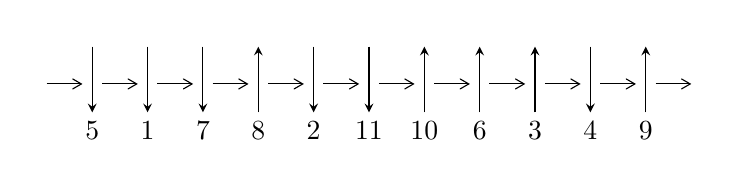
\begin{tikzpicture}[x=20pt, y=17pt]
	% nodes
	\node (C0) at (0, 0) {};
	\node (C1) at (1, 0) {};
	\node (C1U) at (1, +1) {};
	\node (C1D) at (1, -1) {5};

	\node (C2) at (2, 0) {};
	\node (C2U) at (2, +1) {};
	\node (C2D) at (2, -1) {1};

	\node (C3) at (3, 0) {};
	\node (C3U) at (3, +1) {};
	\node (C3D) at (3, -1) {7};

	\node (C4) at (4, 0) {};
	\node (C4U) at (4, +1) {};
	\node (C4D) at (4, -1) {8};

	\node (C5) at (5, 0) {};
	\node (C5U) at (5, +1) {};
	\node (C5D) at (5, -1) {2};

	\node (C6) at (6, 0) {};
	\node (C6U) at (6, +1) {};
	\node (C6D) at (6, -1) {11};

	\node (C7) at (7, 0) {};
	\node (C7U) at (7, +1) {};
	\node (C7D) at (7, -1) {10};

	\node (C8) at (8, 0) {};
	\node (C8U) at (8, +1) {};
	\node (C8D) at (8, -1) {6};

	\node (C9) at (9, 0) {};
	\node (C9U) at (9, +1) {};
	\node (C9D) at (9, -1) {3};

	\node (C10) at (10, 0) {};
	\node (C10U) at (10, +1) {};
	\node (C10D) at (10, -1) {4};

	\node (C11) at (11, 0) {};
	\node (C11U) at (11, +1) {};
	\node (C11D) at (11, -1) {9};
	\node (C12) at (12, 0) {};

	% arrows
	\draw[->,>={angle 60}]
	(C0) edge (C1) (C1) edge (C2) (C2) edge (C3) (C3) edge (C4) (C4) edge (C5) (C5) edge (C6) (C6) edge (C7) (C7) edge (C8) (C8) edge (C9) (C9) edge (C10) (C10) edge (C11) (C11) edge (C12) ;	\draw[->,>=stealth]
	(C1U) edge (C1D) (C2U) edge (C2D) (C3U) edge (C3D) (C4D) edge (C4U) (C5U) edge (C5D) (C6U) edge (C6D) (C7D) edge (C7U) (C8D) edge (C8U) (C9D) edge (C9U) (C10U) edge (C10D) (C11D) edge (C11U) ;
	\end{tikzpicture} \\
\hhline{~~} \\& 
\textbf{Solving Sequence} \\ \cline{2-2} 
 &
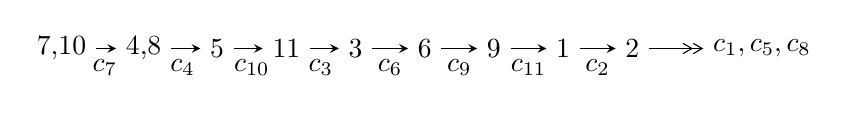
\begin{tikzpicture}[x=25pt, y=7pt]
	% node
	\node (A0) at (-1/8, 0) {7,10};
	\node (A1) at (17/16, 0) {4,8};
	\node (A2) at (17/8, 0) {5};
	\node (A3) at (25/8, 0) {11};
	\node (A4) at (33/8, 0) {3};
	\node (A5) at (41/8, 0) {6};
	\node (A6) at (49/8, 0) {9};
	\node (A7) at (57/8, 0) {1};
	\node (A8) at (65/8, 0) {2};
	\node (C1) at (1/2, -1) {$c_{7}$};
	\node (C2) at (13/8, -1) {$c_{4}$};
	\node (C3) at (21/8, -1) {$c_{10}$};
	\node (C4) at (29/8, -1) {$c_{3}$};
	\node (C5) at (37/8, -1) {$c_{6}$};
	\node (C6) at (45/8, -1) {$c_{9}$};
	\node (C7) at (53/8, -1) {$c_{11}$};
	\node (C8) at (61/8, -1) {$c_{2}$};
	\node (A9) at (10, 0) {$c_{1},c_{5},c_{8}$};

	% edge
	\draw[->,>=stealth]	
	(A0) edge (A1) (A1) edge (A2) (A2) edge (A3) (A3) edge (A4) (A4) edge (A5) (A5) edge (A6) (A6) edge (A7) (A7) edge (A8) ;
	\draw[->>,>={angle 60}]	
	(A8) edge (A9);
\end{tikzpicture} \\ 

\end{tabular} \\

\footnotetext{
The image of knot diagram is generated by the software ``\textbf{Draw programme}" developed by Andrew Bartholomew(\url{http://www.layer8.co.uk/maths/draw/index.htm\#Running-draw}), where we modified some parts for our purpose(\url{https://github.com/CATsTAILs/LinksPainter}).
}\phantom \\ \newline 
\centering \textbf{Ideals for irreducible components\footnotemark of $X_{\text{par}}$} 
 
\begin{align*}
I^u_{1}&=\langle 
-1.47044\times10^{43} u^{38}+4.27047\times10^{44} u^{37}+\cdots+9.58937\times10^{43} b-1.14769\times10^{44},\\
\phantom{I^u_{1}}&\phantom{= \langle  }5.73844\times10^{43} u^{38}-1.63474\times10^{45} u^{37}+\cdots+1.91787\times10^{44} a+3.56267\times10^{43},\;u^{39}-29 u^{38}+\cdots+14 u-4\rangle \\
I^u_{2}&=\langle 
2430 u^{18} a^3-5190 u^{18} a^2+\cdots+12488 a^2-9913,\;24 u^{18} a^3+64 u^{18} a^2+\cdots+58 a+349,\\
\phantom{I^u_{2}}&\phantom{= \langle  }u^{19}+9 u^{18}+\cdots- u-2\rangle \\
I^u_{3}&=\langle 
1560902 u^{18}+15217104 u^{17}+\cdots+4517673 b+1159923,\\
\phantom{I^u_{3}}&\phantom{= \langle  }-386641 u^{18}+43014 u^{17}+\cdots+13553019 a-28935738,\;u^{19}+12 u^{18}+\cdots+51 u+9\rangle \\
\\
I^v_{1}&=\langle 
a,\;b+1,\;v^2- v+1\rangle \\
I^v_{2}&=\langle 
a,\;b+v-1,\;v^2- v+1\rangle \\
\end{align*}
\raggedright * 5 irreducible components of $\dim_{\mathbb{C}}=0$, with total 138 representations.\\
\footnotetext{All coefficients of polynomials are rational numbers. But the coefficients are sometimes approximated in decimal forms when there is not enough margin.}
\newpage
\renewcommand{\arraystretch}{1}
\centering \section*{I. $I^u_{1}= \langle -1.47\times10^{43} u^{38}+4.27\times10^{44} u^{37}+\cdots+9.59\times10^{43} b-1.15\times10^{44},\;5.74\times10^{43} u^{38}-1.63\times10^{45} u^{37}+\cdots+1.92\times10^{44} a+3.56\times10^{43},\;u^{39}-29 u^{38}+\cdots+14 u-4 \rangle$}
\flushleft \textbf{(i) Arc colorings}\\
\begin{tabular}{m{7pt} m{180pt} m{7pt} m{180pt} }
\flushright $a_{7}=$&$\begin{pmatrix}1\\0\end{pmatrix}$ \\
\flushright $a_{10}=$&$\begin{pmatrix}0\\u\end{pmatrix}$ \\
\flushright $a_{4}=$&$\begin{pmatrix}-0.299208 u^{38}+8.52370 u^{37}+\cdots+2.19933 u-0.185762\\0.153341 u^{38}-4.45334 u^{37}+\cdots-4.00316 u+1.19683\end{pmatrix}$ \\
\flushright $a_{8}=$&$\begin{pmatrix}1\\- u^2\end{pmatrix}$ \\
\flushright $a_{5}=$&$\begin{pmatrix}-0.139409 u^{38}+3.92433 u^{37}+\cdots-0.853890 u+0.397710\\0.126095 u^{38}-3.74672 u^{37}+\cdots-4.15512 u+1.05762\end{pmatrix}$ \\
\flushright $a_{11}=$&$\begin{pmatrix}-0.238011 u^{38}+7.00101 u^{37}+\cdots+10.6223 u+0.765363\\-0.0987012 u^{38}+2.65437 u^{37}+\cdots-3.09751 u+0.952043\end{pmatrix}$ \\
\flushright $a_{3}=$&$\begin{pmatrix}-0.145868 u^{38}+4.07037 u^{37}+\cdots-1.80383 u+1.01107\\0.153341 u^{38}-4.45334 u^{37}+\cdots-4.00316 u+1.19683\end{pmatrix}$ \\
\flushright $a_{6}=$&$\begin{pmatrix}-0.0442803 u^{38}+1.19691 u^{37}+\cdots+8.27899 u-3.04017\\0.295182 u^{38}-8.17668 u^{37}+\cdots+1.08639 u+0.571926\end{pmatrix}$ \\
\flushright $a_{9}=$&$\begin{pmatrix}-0.227449 u^{38}+6.41835 u^{37}+\cdots+0.0934401 u+3.06425\\0.109263 u^{38}-3.23703 u^{37}+\cdots-5.43137 u+1.34685\end{pmatrix}$ \\
\flushright $a_{1}=$&$\begin{pmatrix}-0.0331425 u^{38}+1.03976 u^{37}+\cdots+0.307399 u+0.302283\\-0.247066 u^{38}+6.86896 u^{37}+\cdots+0.529326 u-0.320849\end{pmatrix}$ \\
\flushright $a_{2}=$&$\begin{pmatrix}-0.150801 u^{38}+4.40571 u^{37}+\cdots+1.28760 u-0.423103\\-0.240955 u^{38}+6.61929 u^{37}+\cdots-0.756100 u+0.338269\end{pmatrix}$\\ \flushright $a_{2}=$&$\begin{pmatrix}-0.150801 u^{38}+4.40571 u^{37}+\cdots+1.28760 u-0.423103\\-0.240955 u^{38}+6.61929 u^{37}+\cdots-0.756100 u+0.338269\end{pmatrix}$\\&\end{tabular}
\flushleft \textbf{(ii) Obstruction class $= -1$}\\~\\
\flushleft \textbf{(iii) Cusp Shapes $= -1.44324 u^{38}+40.0008 u^{37}+\cdots-2.64538 u-0.932055$}\\~\\
\newpage\renewcommand{\arraystretch}{1}
\flushleft \textbf{(iv) u-Polynomials at the component}\newline \\
\begin{tabular}{m{50pt}|m{274pt}}
Crossings & \hspace{64pt}u-Polynomials at each crossing \\
\hline $$\begin{aligned}c_{1},c_{5}\end{aligned}$$&$\begin{aligned}
&u^{39}+9 u^{38}+\cdots-124 u-16
\end{aligned}$\\
\hline $$\begin{aligned}c_{2}\end{aligned}$$&$\begin{aligned}
&u^{39}+17 u^{38}+\cdots+1200 u+256
\end{aligned}$\\
\hline $$\begin{aligned}c_{3},c_{10}\end{aligned}$$&$\begin{aligned}
&u^{39}-4 u^{37}+\cdots+u-1
\end{aligned}$\\
\hline $$\begin{aligned}c_{4},c_{9}\end{aligned}$$&$\begin{aligned}
&u^{39}- u^{38}+\cdots+47 u+17
\end{aligned}$\\
\hline $$\begin{aligned}c_{6}\end{aligned}$$&$\begin{aligned}
&u^{39}+37 u^{38}+\cdots+5505024 u+262144
\end{aligned}$\\
\hline $$\begin{aligned}c_{7}\end{aligned}$$&$\begin{aligned}
&u^{39}+29 u^{38}+\cdots+14 u+4
\end{aligned}$\\
\hline $$\begin{aligned}c_{8},c_{11}\end{aligned}$$&$\begin{aligned}
&u^{39}- u^{38}+\cdots- u-1
\end{aligned}$\\
\hline
\end{tabular}\\~\\
\newpage\renewcommand{\arraystretch}{1}
\flushleft \textbf{(v) Riley Polynomials at the component}\newline \\
\begin{tabular}{m{50pt}|m{274pt}}
Crossings & \hspace{64pt}Riley Polynomials at each crossing \\
\hline $$\begin{aligned}c_{1},c_{5}\end{aligned}$$&$\begin{aligned}
&y^{39}-17 y^{38}+\cdots+1200 y-256
\end{aligned}$\\
\hline $$\begin{aligned}c_{2}\end{aligned}$$&$\begin{aligned}
&y^{39}+11 y^{38}+\cdots-231680 y-65536
\end{aligned}$\\
\hline $$\begin{aligned}c_{3},c_{10}\end{aligned}$$&$\begin{aligned}
&y^{39}-8 y^{38}+\cdots+9 y-1
\end{aligned}$\\
\hline $$\begin{aligned}c_{4},c_{9}\end{aligned}$$&$\begin{aligned}
&y^{39}-19 y^{38}+\cdots+3399 y-289
\end{aligned}$\\
\hline $$\begin{aligned}c_{6}\end{aligned}$$&$\begin{aligned}
&y^{39}-5 y^{38}+\cdots+515396075520 y-68719476736
\end{aligned}$\\
\hline $$\begin{aligned}c_{7}\end{aligned}$$&$\begin{aligned}
&y^{39}-11 y^{38}+\cdots-276 y-16
\end{aligned}$\\
\hline $$\begin{aligned}c_{8},c_{11}\end{aligned}$$&$\begin{aligned}
&y^{39}+y^{38}+\cdots+37 y-1
\end{aligned}$\\
\hline
\end{tabular}\\~\\
\newpage\flushleft \textbf{(vi) Complex Volumes and Cusp Shapes}
$$\begin{array}{c|c|c}  
\text{Solutions to }I^u_{1}& \I (\text{vol} + \sqrt{-1}CS) & \text{Cusp shape}\\
 \hline 
\begin{aligned}
u &= \phantom{-}0.331870 + 0.943428 I \\
a &= -0.133268 - 0.994133 I \\
b &= -0.893665 + 0.455652 I\end{aligned}
 & -3.26169 - 3.52438 I & \phantom{-0.000000 } 0 \\ \hline\begin{aligned}
u &= \phantom{-}0.331870 - 0.943428 I \\
a &= -0.133268 + 0.994133 I \\
b &= -0.893665 - 0.455652 I\end{aligned}
 & -3.26169 + 3.52438 I & \phantom{-0.000000 } 0 \\ \hline\begin{aligned}
u &= \phantom{-}0.841757 + 0.821032 I \\
a &= -0.625635 - 0.086146 I \\
b &= \phantom{-}0.455904 + 0.586181 I\end{aligned}
 & -1.14633 - 4.05626 I & \phantom{-0.000000 } 0 \\ \hline\begin{aligned}
u &= \phantom{-}0.841757 - 0.821032 I \\
a &= -0.625635 + 0.086146 I \\
b &= \phantom{-}0.455904 - 0.586181 I\end{aligned}
 & -1.14633 + 4.05626 I & \phantom{-0.000000 } 0 \\ \hline\begin{aligned}
u &= \phantom{-}0.817409 + 0.895529 I \\
a &= \phantom{-}0.147866 - 0.842126 I \\
b &= -0.875015 + 0.555944 I\end{aligned}
 & -5.58025 + 3.26982 I & \phantom{-0.000000 } 0 \\ \hline\begin{aligned}
u &= \phantom{-}0.817409 - 0.895529 I \\
a &= \phantom{-}0.147866 + 0.842126 I \\
b &= -0.875015 - 0.555944 I\end{aligned}
 & -5.58025 - 3.26982 I & \phantom{-0.000000 } 0 \\ \hline\begin{aligned}
u &= \phantom{-}0.419302 + 0.634476 I \\
a &= -0.038397 + 1.226960 I \\
b &= \phantom{-}0.794577 - 0.490104 I\end{aligned}
 & -1.48621 + 0.90379 I & -4.25055 - 1.87469 I \\ \hline\begin{aligned}
u &= \phantom{-}0.419302 - 0.634476 I \\
a &= -0.038397 - 1.226960 I \\
b &= \phantom{-}0.794577 + 0.490104 I\end{aligned}
 & -1.48621 - 0.90379 I & -4.25055 + 1.87469 I \\ \hline\begin{aligned}
u &= -0.562878 + 1.206500 I \\
a &= \phantom{-}0.021414 - 0.311325 I \\
b &= -0.363558 - 0.201074 I\end{aligned}
 & \phantom{-}1.74925 - 1.27793 I & \phantom{-0.000000 } 0 \\ \hline\begin{aligned}
u &= -0.562878 - 1.206500 I \\
a &= \phantom{-}0.021414 + 0.311325 I \\
b &= -0.363558 + 0.201074 I\end{aligned}
 & \phantom{-}1.74925 + 1.27793 I & \phantom{-0.000000 } 0\\
 \hline 
 \end{array}$$\newpage$$\begin{array}{c|c|c}  
\text{Solutions to }I^u_{1}& \I (\text{vol} + \sqrt{-1}CS) & \text{Cusp shape}\\
 \hline 
\begin{aligned}
u &= \phantom{-}1.301200 + 0.541325 I \\
a &= -0.372119 + 0.962153 I \\
b &= \phantom{-}1.00504 - 1.05051 I\end{aligned}
 & \phantom{-}4.42472 + 1.39638 I & \phantom{-0.000000 } 0 \\ \hline\begin{aligned}
u &= \phantom{-}1.301200 - 0.541325 I \\
a &= -0.372119 - 0.962153 I \\
b &= \phantom{-}1.00504 + 1.05051 I\end{aligned}
 & \phantom{-}4.42472 - 1.39638 I & \phantom{-0.000000 } 0 \\ \hline\begin{aligned}
u &= \phantom{-}1.09375 + 0.89879 I \\
a &= -0.048210 + 1.101960 I \\
b &= \phantom{-}1.04316 - 1.16194 I\end{aligned}
 & -0.36330 + 10.93520 I & \phantom{-0.000000 } 0 \\ \hline\begin{aligned}
u &= \phantom{-}1.09375 - 0.89879 I \\
a &= -0.048210 - 1.101960 I \\
b &= \phantom{-}1.04316 + 1.16194 I\end{aligned}
 & -0.36330 - 10.93520 I & \phantom{-0.000000 } 0 \\ \hline\begin{aligned}
u &= \phantom{-}1.27453 + 0.71084 I \\
a &= \phantom{-}0.227363 - 1.011290 I \\
b &= -1.00865 + 1.12730 I\end{aligned}
 & \phantom{-}6.38619 + 7.86261 I & \phantom{-0.000000 } 0 \\ \hline\begin{aligned}
u &= \phantom{-}1.27453 - 0.71084 I \\
a &= \phantom{-}0.227363 + 1.011290 I \\
b &= -1.00865 - 1.12730 I\end{aligned}
 & \phantom{-}6.38619 - 7.86261 I & \phantom{-0.000000 } 0 \\ \hline\begin{aligned}
u &= \phantom{-}1.49152\phantom{ +0.000000I} \\
a &= \phantom{-}0.906411\phantom{ +0.000000I} \\
b &= -1.35193\phantom{ +0.000000I}\end{aligned}
 & -6.30934\phantom{ +0.000000I} & \phantom{-0.000000 } 0 \\ \hline\begin{aligned}
u &= -0.034630 + 0.476179 I \\
a &= \phantom{-}0.57531 + 1.32639 I \\
b &= \phantom{-}0.651520 - 0.228017 I\end{aligned}
 & -1.40805 + 0.45537 I & -6.68789 - 0.37229 I \\ \hline\begin{aligned}
u &= -0.034630 - 0.476179 I \\
a &= \phantom{-}0.57531 - 1.32639 I \\
b &= \phantom{-}0.651520 + 0.228017 I\end{aligned}
 & -1.40805 - 0.45537 I & -6.68789 + 0.37229 I \\ \hline\begin{aligned}
u &= -0.305932 + 0.311045 I \\
a &= \phantom{-}1.08603 + 1.91133 I \\
b &= \phantom{-}0.926761 + 0.246934 I\end{aligned}
 & -0.07010 - 4.24589 I & -2.71126 + 7.01324 I\\
 \hline 
 \end{array}$$\newpage$$\begin{array}{c|c|c}  
\text{Solutions to }I^u_{1}& \I (\text{vol} + \sqrt{-1}CS) & \text{Cusp shape}\\
 \hline 
\begin{aligned}
u &= -0.305932 - 0.311045 I \\
a &= \phantom{-}1.08603 - 1.91133 I \\
b &= \phantom{-}0.926761 - 0.246934 I\end{aligned}
 & -0.07010 + 4.24589 I & -2.71126 - 7.01324 I \\ \hline\begin{aligned}
u &= \phantom{-}0.166848 + 0.352846 I \\
a &= \phantom{-}0.73742 + 2.79209 I \\
b &= \phantom{-}0.862139 - 0.726050 I\end{aligned}
 & -0.162274 + 0.211332 I & -1.308088 + 0.536675 I \\ \hline\begin{aligned}
u &= \phantom{-}0.166848 - 0.352846 I \\
a &= \phantom{-}0.73742 - 2.79209 I \\
b &= \phantom{-}0.862139 + 0.726050 I\end{aligned}
 & -0.162274 - 0.211332 I & -1.308088 - 0.536675 I \\ \hline\begin{aligned}
u &= \phantom{-}1.24696 + 1.01994 I \\
a &= \phantom{-}0.026843 - 0.978351 I \\
b &= -1.03133 + 1.19259 I\end{aligned}
 & \phantom{-}6.6772 + 13.2005 I & \phantom{-0.000000 } 0 \\ \hline\begin{aligned}
u &= \phantom{-}1.24696 - 1.01994 I \\
a &= \phantom{-}0.026843 + 0.978351 I \\
b &= -1.03133 - 1.19259 I\end{aligned}
 & \phantom{-}6.6772 - 13.2005 I & \phantom{-0.000000 } 0 \\ \hline\begin{aligned}
u &= \phantom{-}1.22434 + 1.08925 I \\
a &= \phantom{-}0.011484 + 0.970890 I \\
b &= \phantom{-}1.04348 - 1.20121 I\end{aligned}
 & \phantom{-}4.8624 + 19.2051 I & \phantom{-0.000000 } 0 \\ \hline\begin{aligned}
u &= \phantom{-}1.22434 - 1.08925 I \\
a &= \phantom{-}0.011484 - 0.970890 I \\
b &= \phantom{-}1.04348 + 1.20121 I\end{aligned}
 & \phantom{-}4.8624 - 19.2051 I & \phantom{-0.000000 } 0 \\ \hline\begin{aligned}
u &= -0.318547 + 0.066288 I \\
a &= -2.76662 - 1.78349 I \\
b &= -0.999521 - 0.384730 I\end{aligned}
 & \phantom{-}0.0975477 - 0.0620158 I & -2.09239 + 0.09201 I \\ \hline\begin{aligned}
u &= -0.318547 - 0.066288 I \\
a &= -2.76662 + 1.78349 I \\
b &= -0.999521 + 0.384730 I\end{aligned}
 & \phantom{-}0.0975477 + 0.0620158 I & -2.09239 - 0.09201 I \\ \hline\begin{aligned}
u &= -0.103070 + 0.291494 I \\
a &= -2.92237 - 2.35332 I \\
b &= -0.987188 + 0.609296 I\end{aligned}
 & -0.09530 + 3.97123 I & -1.67802 - 6.97168 I\\
 \hline 
 \end{array}$$\newpage$$\begin{array}{c|c|c}  
\text{Solutions to }I^u_{1}& \I (\text{vol} + \sqrt{-1}CS) & \text{Cusp shape}\\
 \hline 
\begin{aligned}
u &= -0.103070 - 0.291494 I \\
a &= -2.92237 + 2.35332 I \\
b &= -0.987188 - 0.609296 I\end{aligned}
 & -0.09530 - 3.97123 I & -1.67802 + 6.97168 I \\ \hline\begin{aligned}
u &= \phantom{-}1.76013 + 0.77135 I \\
a &= -0.314047 + 0.368852 I \\
b &= \phantom{-}0.837278 - 0.406987 I\end{aligned}
 & \phantom{-}2.84675 + 3.80672 I & \phantom{-0.000000 } 0 \\ \hline\begin{aligned}
u &= \phantom{-}1.76013 - 0.77135 I \\
a &= -0.314047 - 0.368852 I \\
b &= \phantom{-}0.837278 + 0.406987 I\end{aligned}
 & \phantom{-}2.84675 - 3.80672 I & \phantom{-0.000000 } 0 \\ \hline\begin{aligned}
u &= \phantom{-}1.62789 + 1.03730 I \\
a &= \phantom{-}0.210948 - 0.444220 I \\
b &= -0.804192 + 0.504323 I\end{aligned}
 & \phantom{-}1.25508 + 10.27040 I & \phantom{-0.000000 } 0 \\ \hline\begin{aligned}
u &= \phantom{-}1.62789 - 1.03730 I \\
a &= \phantom{-}0.210948 + 0.444220 I \\
b &= -0.804192 - 0.504323 I\end{aligned}
 & \phantom{-}1.25508 - 10.27040 I & \phantom{-0.000000 } 0 \\ \hline\begin{aligned}
u &= \phantom{-}1.55330 + 1.50941 I \\
a &= -0.261427 - 0.177739 I \\
b &= \phantom{-}0.137795 + 0.670683 I\end{aligned}
 & \phantom{-}4.32938 - 9.77720 I & \phantom{-0.000000 } 0 \\ \hline\begin{aligned}
u &= \phantom{-}1.55330 - 1.50941 I \\
a &= -0.261427 + 0.177739 I \\
b &= \phantom{-}0.137795 - 0.670683 I\end{aligned}
 & \phantom{-}4.32938 + 9.77720 I & \phantom{-0.000000 } 0 \\ \hline\begin{aligned}
u &= \phantom{-}1.42000 + 1.74003 I \\
a &= \phantom{-}0.234216 + 0.122995 I \\
b &= -0.118571 - 0.582195 I\end{aligned}
 & \phantom{-}5.48378 - 3.90827 I & \phantom{-0.000000 } 0 \\ \hline\begin{aligned}
u &= \phantom{-}1.42000 - 1.74003 I \\
a &= \phantom{-}0.234216 - 0.122995 I \\
b &= -0.118571 + 0.582195 I\end{aligned}
 & \phantom{-}5.48378 + 3.90827 I & \phantom{-0.000000 } 0\\
 \hline 
 \end{array}$$\newpage\newpage\renewcommand{\arraystretch}{1}
\centering \section*{II. $I^u_{2}= \langle 2430 u^{18} a^3-5190 u^{18} a^2+\cdots+12488 a^2-9913,\;24 u^{18} a^3+64 u^{18} a^2+\cdots+58 a+349,\;u^{19}+9 u^{18}+\cdots- u-2 \rangle$}
\flushleft \textbf{(i) Arc colorings}\\
\begin{tabular}{m{7pt} m{180pt} m{7pt} m{180pt} }
\flushright $a_{7}=$&$\begin{pmatrix}1\\0\end{pmatrix}$ \\
\flushright $a_{10}=$&$\begin{pmatrix}0\\u\end{pmatrix}$ \\
\flushright $a_{4}=$&$\begin{pmatrix}a\\-0.332968 a^{3} u^{18}+0.711154 a^{2} u^{18}+\cdots-1.71115 a^{2}+1.35832\end{pmatrix}$ \\
\flushright $a_{8}=$&$\begin{pmatrix}1\\- u^2\end{pmatrix}$ \\
\flushright $a_{5}=$&$\begin{pmatrix}-0.332968 a^{3} u^{18}+0.711154 a^{2} u^{18}+\cdots+a+1.35832\\-1.00110 a^{3} u^{18}-0.133461 a^{2} u^{18}+\cdots+1.13346 a^{2}+1.92505\end{pmatrix}$ \\
\flushright $a_{11}=$&$\begin{pmatrix}- a^2 u\\0.711154 a^{3} u^{18}+0.332968 a^{2} u^{18}+\cdots-4 a-0.999863\end{pmatrix}$ \\
\flushright $a_{3}=$&$\begin{pmatrix}-0.332968 a^{3} u^{18}+0.711154 a^{2} u^{18}+\cdots+a+1.35832\\-0.332968 a^{3} u^{18}+0.711154 a^{2} u^{18}+\cdots-1.71115 a^{2}+1.35832\end{pmatrix}$ \\
\flushright $a_{6}=$&$\begin{pmatrix}-0.144423 a^{3} u^{18}-0.333516 a^{2} u^{18}+\cdots-0.666484 a^{2}+0.500069\\0.711154 a^{3} u^{18}+0.332968 a^{2} u^{18}+\cdots-4 a+0.000137024\end{pmatrix}$ \\
\flushright $a_{9}=$&$\begin{pmatrix}0.155385 a^{3} u^{18}+0.668128 a^{2} u^{18}+\cdots-0.668128 a^{2}-0.000548095\\-0.555769 a^{3} u^{18}+0.335160 a^{2} u^{18}+\cdots+4 a+0.999315\end{pmatrix}$ \\
\flushright $a_{1}=$&$\begin{pmatrix}-0.411346 a^{3} u^{18}+0.668676 a^{2} u^{18}+\cdots-0.668676 a^{2}+0.499246\\-0.133461 a^{3} u^{18}+1.00110 a^{2} u^{18}+\cdots-2 a-0.000411072\end{pmatrix}$ \\
\flushright $a_{2}=$&$\begin{pmatrix}-0.676350 a^{3} u^{18}+0.654426 a^{2} u^{18}+\cdots-a+1.50459\\-0.338449 a^{3} u^{18}+1.04385 a^{2} u^{18}+\cdots-6 a+0.983557\end{pmatrix}$\\ \flushright $a_{2}=$&$\begin{pmatrix}-0.676350 a^{3} u^{18}+0.654426 a^{2} u^{18}+\cdots-a+1.50459\\-0.338449 a^{3} u^{18}+1.04385 a^{2} u^{18}+\cdots-6 a+0.983557\end{pmatrix}$\\&\end{tabular}
\flushleft \textbf{(ii) Obstruction class $= -1$}\\~\\
\flushleft \textbf{(iii) Cusp Shapes $= -\frac{10380}{3649} u^{18} a^3-\frac{4860}{3649} u^{18} a^2+\cdots+16 a+\frac{62031}{3649}$}\\~\\
\newpage\renewcommand{\arraystretch}{1}
\flushleft \textbf{(iv) u-Polynomials at the component}\newline \\
\begin{tabular}{m{50pt}|m{274pt}}
Crossings & \hspace{64pt}u-Polynomials at each crossing \\
\hline $$\begin{aligned}c_{1},c_{5}\end{aligned}$$&$\begin{aligned}
&(u^{19}-2 u^{18}+\cdots-4 u+1)^{4}
\end{aligned}$\\
\hline $$\begin{aligned}c_{2}\end{aligned}$$&$\begin{aligned}
&(u^{19}+8 u^{18}+\cdots+4 u+1)^{4}
\end{aligned}$\\
\hline $$\begin{aligned}c_{3},c_{10}\end{aligned}$$&$\begin{aligned}
&u^{76}+4 u^{75}+\cdots-13 u+1
\end{aligned}$\\
\hline $$\begin{aligned}c_{4},c_{9}\end{aligned}$$&$\begin{aligned}
&u^{76}+2 u^{75}+\cdots-461147 u+92641
\end{aligned}$\\
\hline $$\begin{aligned}c_{6}\end{aligned}$$&$\begin{aligned}
&(u^2- u+1)^{38}
\end{aligned}$\\
\hline $$\begin{aligned}c_{7}\end{aligned}$$&$\begin{aligned}
&(u^{19}-9 u^{18}+\cdots- u+2)^{4}
\end{aligned}$\\
\hline $$\begin{aligned}c_{8},c_{11}\end{aligned}$$&$\begin{aligned}
&u^{76}-3 u^{75}+\cdots+7318 u+1741
\end{aligned}$\\
\hline
\end{tabular}\\~\\
\newpage\renewcommand{\arraystretch}{1}
\flushleft \textbf{(v) Riley Polynomials at the component}\newline \\
\begin{tabular}{m{50pt}|m{274pt}}
Crossings & \hspace{64pt}Riley Polynomials at each crossing \\
\hline $$\begin{aligned}c_{1},c_{5}\end{aligned}$$&$\begin{aligned}
&(y^{19}-8 y^{18}+\cdots+4 y-1)^{4}
\end{aligned}$\\
\hline $$\begin{aligned}c_{2}\end{aligned}$$&$\begin{aligned}
&(y^{19}+8 y^{18}+\cdots-16 y-1)^{4}
\end{aligned}$\\
\hline $$\begin{aligned}c_{3},c_{10}\end{aligned}$$&$\begin{aligned}
&y^{76}+26 y^{75}+\cdots+75 y+1
\end{aligned}$\\
\hline $$\begin{aligned}c_{4},c_{9}\end{aligned}$$&$\begin{aligned}
&y^{76}-34 y^{75}+\cdots-289799457437 y+8582354881
\end{aligned}$\\
\hline $$\begin{aligned}c_{6}\end{aligned}$$&$\begin{aligned}
&(y^2+y+1)^{38}
\end{aligned}$\\
\hline $$\begin{aligned}c_{7}\end{aligned}$$&$\begin{aligned}
&(y^{19}-3 y^{18}+\cdots+37 y-4)^{4}
\end{aligned}$\\
\hline $$\begin{aligned}c_{8},c_{11}\end{aligned}$$&$\begin{aligned}
&y^{76}-31 y^{75}+\cdots-27023766 y+3031081
\end{aligned}$\\
\hline
\end{tabular}\\~\\
\newpage\flushleft \textbf{(vi) Complex Volumes and Cusp Shapes}
$$\begin{array}{c|c|c}  
\text{Solutions to }I^u_{2}& \I (\text{vol} + \sqrt{-1}CS) & \text{Cusp shape}\\
 \hline 
\begin{aligned}
u &= -0.488744 + 1.038280 I \\
a &= -0.046618 + 0.988356 I \\
b &= -0.79374 - 1.47743 I\end{aligned}
 & \phantom{-}0.05398 - 9.62803 I & -3.53397 + 12.41778 I \\ \hline\begin{aligned}
u &= -0.488744 + 1.038280 I \\
a &= -0.293242 + 0.933326 I \\
b &= -0.111329 - 0.106061 I\end{aligned}
 & \phantom{-}0.05398 - 5.56826 I & -3.53397 + 5.48958 I \\ \hline\begin{aligned}
u &= -0.488744 + 1.038280 I \\
a &= \phantom{-}0.87027 - 1.17413 I \\
b &= \phantom{-}1.003410 + 0.531456 I\end{aligned}
 & \phantom{-}0.05398 - 9.62803 I & -3.53397 + 12.41778 I \\ \hline\begin{aligned}
u &= -0.488744 + 1.038280 I \\
a &= \phantom{-}0.0423036 - 0.1271370 I \\
b &= \phantom{-}0.825736 + 0.760626 I\end{aligned}
 & \phantom{-}0.05398 - 5.56826 I & -3.53397 + 5.48958 I \\ \hline\begin{aligned}
u &= -0.488744 - 1.038280 I \\
a &= -0.046618 - 0.988356 I \\
b &= -0.79374 + 1.47743 I\end{aligned}
 & \phantom{-}0.05398 + 9.62803 I & -3.53397 - 12.41778 I \\ \hline\begin{aligned}
u &= -0.488744 - 1.038280 I \\
a &= -0.293242 - 0.933326 I \\
b &= -0.111329 + 0.106061 I\end{aligned}
 & \phantom{-}0.05398 + 5.56826 I & -3.53397 - 5.48958 I \\ \hline\begin{aligned}
u &= -0.488744 - 1.038280 I \\
a &= \phantom{-}0.87027 + 1.17413 I \\
b &= \phantom{-}1.003410 - 0.531456 I\end{aligned}
 & \phantom{-}0.05398 + 9.62803 I & -3.53397 - 12.41778 I \\ \hline\begin{aligned}
u &= -0.488744 - 1.038280 I \\
a &= \phantom{-}0.0423036 + 0.1271370 I \\
b &= \phantom{-}0.825736 - 0.760626 I\end{aligned}
 & \phantom{-}0.05398 + 5.56826 I & -3.53397 - 5.48958 I \\ \hline\begin{aligned}
u &= -0.752606 + 0.874521 I \\
a &= \phantom{-}0.009232 - 0.929025 I \\
b &= \phantom{-}0.89425 + 1.37563 I\end{aligned}
 & \phantom{-}1.75286 - 5.17897 I & \phantom{-}0.41778 + 7.25838 I \\ \hline\begin{aligned}
u &= -0.752606 + 0.874521 I \\
a &= \phantom{-}0.130623 - 0.587298 I \\
b &= -0.207899 + 0.298912 I\end{aligned}
 & \phantom{-}1.75286 - 1.11920 I & \phantom{-}0.417778 + 0.330175 I\\
 \hline 
 \end{array}$$\newpage$$\begin{array}{c|c|c}  
\text{Solutions to }I^u_{2}& \I (\text{vol} + \sqrt{-1}CS) & \text{Cusp shape}\\
 \hline 
\begin{aligned}
u &= -0.752606 + 0.874521 I \\
a &= -0.39813 + 1.36519 I \\
b &= -0.805505 - 0.707263 I\end{aligned}
 & \phantom{-}1.75286 - 5.17897 I & \phantom{-}0.41778 + 7.25838 I \\ \hline\begin{aligned}
u &= -0.752606 + 0.874521 I \\
a &= -0.313905 + 0.032415 I \\
b &= -0.415297 - 0.556237 I\end{aligned}
 & \phantom{-}1.75286 - 1.11920 I & \phantom{-}0.417778 + 0.330175 I \\ \hline\begin{aligned}
u &= -0.752606 - 0.874521 I \\
a &= \phantom{-}0.009232 + 0.929025 I \\
b &= \phantom{-}0.89425 - 1.37563 I\end{aligned}
 & \phantom{-}1.75286 + 5.17897 I & \phantom{-}0.41778 - 7.25838 I \\ \hline\begin{aligned}
u &= -0.752606 - 0.874521 I \\
a &= \phantom{-}0.130623 + 0.587298 I \\
b &= -0.207899 - 0.298912 I\end{aligned}
 & \phantom{-}1.75286 + 1.11920 I & \phantom{-}0.417778 - 0.330175 I \\ \hline\begin{aligned}
u &= -0.752606 - 0.874521 I \\
a &= -0.39813 - 1.36519 I \\
b &= -0.805505 + 0.707263 I\end{aligned}
 & \phantom{-}1.75286 + 5.17897 I & \phantom{-}0.41778 - 7.25838 I \\ \hline\begin{aligned}
u &= -0.752606 - 0.874521 I \\
a &= -0.313905 - 0.032415 I \\
b &= -0.415297 + 0.556237 I\end{aligned}
 & \phantom{-}1.75286 + 1.11920 I & \phantom{-}0.417778 - 0.330175 I \\ \hline\begin{aligned}
u &= -1.211130 + 0.137559 I \\
a &= -0.836689 + 0.841595 I \\
b &= \phantom{-}0.089876 - 0.698008 I\end{aligned}
 & \phantom{-}4.59520 - 0.63634 I & \phantom{-}7.58619 - 0.25531 I \\ \hline\begin{aligned}
u &= -1.211130 + 0.137559 I \\
a &= \phantom{-}0.695655 + 1.094640 I \\
b &= -0.211353 - 0.748765 I\end{aligned}
 & \phantom{-}4.59520 - 4.69611 I & \phantom{-}7.58619 + 6.67289 I \\ \hline\begin{aligned}
u &= -1.211130 + 0.137559 I \\
a &= -0.102962 - 0.629929 I \\
b &= \phantom{-}0.99311 + 1.23007 I\end{aligned}
 & \phantom{-}4.59520 - 4.69611 I & \phantom{-}7.58619 + 6.67289 I \\ \hline\begin{aligned}
u &= -1.211130 + 0.137559 I \\
a &= \phantom{-}0.137888 - 0.560665 I \\
b &= -0.89757 + 1.13438 I\end{aligned}
 & \phantom{-}4.59520 - 0.63634 I & \phantom{-}7.58619 - 0.25531 I\\
 \hline 
 \end{array}$$\newpage$$\begin{array}{c|c|c}  
\text{Solutions to }I^u_{2}& \I (\text{vol} + \sqrt{-1}CS) & \text{Cusp shape}\\
 \hline 
\begin{aligned}
u &= -1.211130 - 0.137559 I \\
a &= -0.836689 - 0.841595 I \\
b &= \phantom{-}0.089876 + 0.698008 I\end{aligned}
 & \phantom{-}4.59520 + 0.63634 I & \phantom{-}7.58619 + 0.25531 I \\ \hline\begin{aligned}
u &= -1.211130 - 0.137559 I \\
a &= \phantom{-}0.695655 - 1.094640 I \\
b &= -0.211353 + 0.748765 I\end{aligned}
 & \phantom{-}4.59520 + 4.69611 I & \phantom{-}7.58619 - 6.67289 I \\ \hline\begin{aligned}
u &= -1.211130 - 0.137559 I \\
a &= -0.102962 + 0.629929 I \\
b &= \phantom{-}0.99311 - 1.23007 I\end{aligned}
 & \phantom{-}4.59520 + 4.69611 I & \phantom{-}7.58619 - 6.67289 I \\ \hline\begin{aligned}
u &= -1.211130 - 0.137559 I \\
a &= \phantom{-}0.137888 + 0.560665 I \\
b &= -0.89757 - 1.13438 I\end{aligned}
 & \phantom{-}4.59520 + 0.63634 I & \phantom{-}7.58619 + 0.25531 I \\ \hline\begin{aligned}
u &= \phantom{-}0.687103 + 0.235969 I \\
a &= \phantom{-}0.041834 - 0.923046 I \\
b &= \phantom{-}1.52253 + 1.30009 I\end{aligned}
 & \phantom{-}4.06740 + 10.25010 I & \phantom{-}5.86786 - 12.03410 I \\ \hline\begin{aligned}
u &= \phantom{-}0.687103 + 0.235969 I \\
a &= \phantom{-}0.61351 + 1.33915 I \\
b &= \phantom{-}1.13417 - 1.00234 I\end{aligned}
 & \phantom{-}4.06740 + 6.19033 I & \phantom{-}5.86786 - 5.10589 I \\ \hline\begin{aligned}
u &= \phantom{-}0.687103 + 0.235969 I \\
a &= -1.02838 + 1.81197 I \\
b &= -0.105545 - 1.064900 I\end{aligned}
 & \phantom{-}4.06740 + 6.19033 I & \phantom{-}5.86786 - 5.10589 I \\ \hline\begin{aligned}
u &= \phantom{-}0.687103 + 0.235969 I \\
a &= -2.56334 - 1.01181 I \\
b &= -0.246555 + 0.624356 I\end{aligned}
 & \phantom{-}4.06740 + 10.25010 I & \phantom{-}5.86786 - 12.03410 I \\ \hline\begin{aligned}
u &= \phantom{-}0.687103 - 0.235969 I \\
a &= \phantom{-}0.041834 + 0.923046 I \\
b &= \phantom{-}1.52253 - 1.30009 I\end{aligned}
 & \phantom{-}4.06740 - 10.25010 I & \phantom{-}5.86786 + 12.03410 I \\ \hline\begin{aligned}
u &= \phantom{-}0.687103 - 0.235969 I \\
a &= \phantom{-}0.61351 - 1.33915 I \\
b &= \phantom{-}1.13417 + 1.00234 I\end{aligned}
 & \phantom{-}4.06740 - 6.19033 I & \phantom{-}5.86786 + 5.10589 I\\
 \hline 
 \end{array}$$\newpage$$\begin{array}{c|c|c}  
\text{Solutions to }I^u_{2}& \I (\text{vol} + \sqrt{-1}CS) & \text{Cusp shape}\\
 \hline 
\begin{aligned}
u &= \phantom{-}0.687103 - 0.235969 I \\
a &= -1.02838 - 1.81197 I \\
b &= -0.105545 + 1.064900 I\end{aligned}
 & \phantom{-}4.06740 - 6.19033 I & \phantom{-}5.86786 + 5.10589 I \\ \hline\begin{aligned}
u &= \phantom{-}0.687103 - 0.235969 I \\
a &= -2.56334 + 1.01181 I \\
b &= -0.246555 - 0.624356 I\end{aligned}
 & \phantom{-}4.06740 - 10.25010 I & \phantom{-}5.86786 + 12.03410 I \\ \hline\begin{aligned}
u &= \phantom{-}0.689008 + 0.139635 I \\
a &= -0.095129 + 1.010870 I \\
b &= -1.45640 - 1.29970 I\end{aligned}
 & \phantom{-}5.90964 + 4.35931 I & \phantom{-}9.40004 - 6.47018 I \\ \hline\begin{aligned}
u &= \phantom{-}0.689008 + 0.139635 I \\
a &= -0.409287 - 1.280010 I \\
b &= -1.19567 + 1.13465 I\end{aligned}
 & \phantom{-}5.90964 + 0.29954 I & \phantom{-}9.40004 + 0.45802 I \\ \hline\begin{aligned}
u &= \phantom{-}0.689008 + 0.139635 I \\
a &= \phantom{-}1.34631 - 1.91963 I \\
b &= \phantom{-}0.103269 + 0.939085 I\end{aligned}
 & \phantom{-}5.90964 + 0.29954 I & \phantom{-}9.40004 + 0.45802 I \\ \hline\begin{aligned}
u &= \phantom{-}0.689008 + 0.139635 I \\
a &= \phantom{-}2.39759 + 1.40044 I \\
b &= \phantom{-}0.206697 - 0.683213 I\end{aligned}
 & \phantom{-}5.90964 + 4.35931 I & \phantom{-}9.40004 - 6.47018 I \\ \hline\begin{aligned}
u &= \phantom{-}0.689008 - 0.139635 I \\
a &= -0.095129 - 1.010870 I \\
b &= -1.45640 + 1.29970 I\end{aligned}
 & \phantom{-}5.90964 - 4.35931 I & \phantom{-}9.40004 + 6.47018 I \\ \hline\begin{aligned}
u &= \phantom{-}0.689008 - 0.139635 I \\
a &= -0.409287 + 1.280010 I \\
b &= -1.19567 - 1.13465 I\end{aligned}
 & \phantom{-}5.90964 - 0.29954 I & \phantom{-}9.40004 - 0.45802 I \\ \hline\begin{aligned}
u &= \phantom{-}0.689008 - 0.139635 I \\
a &= \phantom{-}1.34631 + 1.91963 I \\
b &= \phantom{-}0.103269 - 0.939085 I\end{aligned}
 & \phantom{-}5.90964 - 0.29954 I & \phantom{-}9.40004 - 0.45802 I \\ \hline\begin{aligned}
u &= \phantom{-}0.689008 - 0.139635 I \\
a &= \phantom{-}2.39759 - 1.40044 I \\
b &= \phantom{-}0.206697 + 0.683213 I\end{aligned}
 & \phantom{-}5.90964 - 4.35931 I & \phantom{-}9.40004 + 6.47018 I\\
 \hline 
 \end{array}$$\newpage$$\begin{array}{c|c|c}  
\text{Solutions to }I^u_{2}& \I (\text{vol} + \sqrt{-1}CS) & \text{Cusp shape}\\
 \hline 
\begin{aligned}
u &= -0.378245 + 0.567353 I \\
a &= \phantom{-}0.131552 + 1.078100 I \\
b &= -1.01749 - 1.65463 I\end{aligned}
 & -2.19784 - 2.79119 I & -7.49818 + 10.51788 I \\ \hline\begin{aligned}
u &= -0.378245 + 0.567353 I \\
a &= -0.324334 + 0.098555 I \\
b &= \phantom{-}1.389240 + 0.131080 I\end{aligned}
 & -2.19784 + 1.26857 I & -7.49818 + 3.58967 I \\ \hline\begin{aligned}
u &= -0.378245 + 0.567353 I \\
a &= \phantom{-}0.97020 + 1.80181 I \\
b &= -0.066762 + 0.221290 I\end{aligned}
 & -2.19784 + 1.26857 I & -7.49818 + 3.58967 I \\ \hline\begin{aligned}
u &= -0.378245 + 0.567353 I \\
a &= \phantom{-}1.19128 - 2.58761 I \\
b &= \phantom{-}0.661419 + 0.333147 I\end{aligned}
 & -2.19784 - 2.79119 I & -7.49818 + 10.51788 I \\ \hline\begin{aligned}
u &= -0.378245 - 0.567353 I \\
a &= \phantom{-}0.131552 - 1.078100 I \\
b &= -1.01749 + 1.65463 I\end{aligned}
 & -2.19784 + 2.79119 I & -7.49818 - 10.51788 I \\ \hline\begin{aligned}
u &= -0.378245 - 0.567353 I \\
a &= -0.324334 - 0.098555 I \\
b &= \phantom{-}1.389240 - 0.131080 I\end{aligned}
 & -2.19784 - 1.26857 I & -7.49818 - 3.58967 I \\ \hline\begin{aligned}
u &= -0.378245 - 0.567353 I \\
a &= \phantom{-}0.97020 - 1.80181 I \\
b &= -0.066762 - 0.221290 I\end{aligned}
 & -2.19784 - 1.26857 I & -7.49818 - 3.58967 I \\ \hline\begin{aligned}
u &= -0.378245 - 0.567353 I \\
a &= \phantom{-}1.19128 + 2.58761 I \\
b &= \phantom{-}0.661419 - 0.333147 I\end{aligned}
 & -2.19784 + 2.79119 I & -7.49818 - 10.51788 I \\ \hline\begin{aligned}
u &= -0.865146 + 1.042810 I \\
a &= \phantom{-}0.045926 - 0.937417 I \\
b &= \phantom{-}0.80203 + 1.30087 I\end{aligned}
 & \phantom{-}1.73711 - 5.29191 I & -1.82857 + 8.05106 I \\ \hline\begin{aligned}
u &= -0.865146 + 1.042810 I \\
a &= -0.360952 + 1.068560 I \\
b &= -0.937819 - 0.858895 I\end{aligned}
 & \phantom{-}1.73711 - 5.29191 I & -1.82857 + 8.05106 I\\
 \hline 
 \end{array}$$\newpage$$\begin{array}{c|c|c}  
\text{Solutions to }I^u_{2}& \I (\text{vol} + \sqrt{-1}CS) & \text{Cusp shape}\\
 \hline 
\begin{aligned}
u &= -0.865146 + 1.042810 I \\
a &= \phantom{-}0.296569 - 0.571023 I \\
b &= \phantom{-}0.024029 + 0.464704 I\end{aligned}
 & \phantom{-}1.73711 - 1.23215 I & -1.82857 + 1.12286 I \\ \hline\begin{aligned}
u &= -0.865146 + 1.042810 I \\
a &= -0.252629 + 0.232631 I \\
b &= -0.338895 - 0.803284 I\end{aligned}
 & \phantom{-}1.73711 - 1.23215 I & -1.82857 + 1.12286 I \\ \hline\begin{aligned}
u &= -0.865146 - 1.042810 I \\
a &= \phantom{-}0.045926 + 0.937417 I \\
b &= \phantom{-}0.80203 - 1.30087 I\end{aligned}
 & \phantom{-}1.73711 + 5.29191 I & -1.82857 - 8.05106 I \\ \hline\begin{aligned}
u &= -0.865146 - 1.042810 I \\
a &= -0.360952 - 1.068560 I \\
b &= -0.937819 + 0.858895 I\end{aligned}
 & \phantom{-}1.73711 + 5.29191 I & -1.82857 - 8.05106 I \\ \hline\begin{aligned}
u &= -0.865146 - 1.042810 I \\
a &= \phantom{-}0.296569 + 0.571023 I \\
b &= \phantom{-}0.024029 - 0.464704 I\end{aligned}
 & \phantom{-}1.73711 + 1.23215 I & -1.82857 - 1.12286 I \\ \hline\begin{aligned}
u &= -0.865146 - 1.042810 I \\
a &= -0.252629 - 0.232631 I \\
b &= -0.338895 + 0.803284 I\end{aligned}
 & \phantom{-}1.73711 + 1.23215 I & -1.82857 - 1.12286 I \\ \hline\begin{aligned}
u &= \phantom{-}0.494703\phantom{ +0.000000I} \\
a &= -0.050248 + 1.334190 I \\
b &= \phantom{-}1.25357 - 1.55428 I\end{aligned}
 & -0.73172 - 2.02988 I & \phantom{-}13.11408 + 3.46410 I \\ \hline\begin{aligned}
u &= \phantom{-}0.494703\phantom{ +0.000000I} \\
a &= -0.050248 - 1.334190 I \\
b &= \phantom{-}1.25357 + 1.55428 I\end{aligned}
 & -0.73172 + 2.02988 I & \phantom{-}13.11408 - 3.46410 I \\ \hline\begin{aligned}
u &= \phantom{-}0.494703\phantom{ +0.000000I} \\
a &= -2.53399 + 3.14184 I \\
b &= \phantom{-}0.024858 - 0.660026 I\end{aligned}
 & -0.73172 - 2.02988 I & \phantom{-}13.11408 + 3.46410 I \\ \hline\begin{aligned}
u &= \phantom{-}0.494703\phantom{ +0.000000I} \\
a &= -2.53399 - 3.14184 I \\
b &= \phantom{-}0.024858 + 0.660026 I\end{aligned}
 & -0.73172 + 2.02988 I & \phantom{-}13.11408 - 3.46410 I\\
 \hline 
 \end{array}$$\newpage$$\begin{array}{c|c|c}  
\text{Solutions to }I^u_{2}& \I (\text{vol} + \sqrt{-1}CS) & \text{Cusp shape}\\
 \hline 
\begin{aligned}
u &= -1.23842 + 1.01885 I \\
a &= \phantom{-}0.057902 + 1.004440 I \\
b &= -0.547319 - 1.129000 I\end{aligned}
 & \phantom{-}4.33121 - 3.93186 I & \phantom{-}7.62421 + 4.84403 I \\ \hline\begin{aligned}
u &= -1.23842 + 1.01885 I \\
a &= \phantom{-}0.183718 - 0.760502 I \\
b &= \phantom{-}1.09508 + 1.18492 I\end{aligned}
 & \phantom{-}4.33121 - 3.93186 I & \phantom{-}7.62421 + 4.84403 I \\ \hline\begin{aligned}
u &= -1.23842 + 1.01885 I \\
a &= -0.490134 + 0.482986 I \\
b &= -0.207412 - 0.651096 I\end{aligned}
 & \phantom{-}4.33121 + 0.12791 I & \phantom{-}7.62421 - 2.08417 I \\ \hline\begin{aligned}
u &= -1.23842 + 1.01885 I \\
a &= \phantom{-}0.158068 - 0.395706 I \\
b &= -0.114899 + 1.097510 I\end{aligned}
 & \phantom{-}4.33121 + 0.12791 I & \phantom{-}7.62421 - 2.08417 I \\ \hline\begin{aligned}
u &= -1.23842 - 1.01885 I \\
a &= \phantom{-}0.057902 - 1.004440 I \\
b &= -0.547319 + 1.129000 I\end{aligned}
 & \phantom{-}4.33121 + 3.93186 I & \phantom{-}7.62421 - 4.84403 I \\ \hline\begin{aligned}
u &= -1.23842 - 1.01885 I \\
a &= \phantom{-}0.183718 + 0.760502 I \\
b &= \phantom{-}1.09508 - 1.18492 I\end{aligned}
 & \phantom{-}4.33121 + 3.93186 I & \phantom{-}7.62421 - 4.84403 I \\ \hline\begin{aligned}
u &= -1.23842 - 1.01885 I \\
a &= -0.490134 - 0.482986 I \\
b &= -0.207412 + 0.651096 I\end{aligned}
 & \phantom{-}4.33121 - 0.12791 I & \phantom{-}7.62421 + 2.08417 I \\ \hline\begin{aligned}
u &= -1.23842 - 1.01885 I \\
a &= \phantom{-}0.158068 + 0.395706 I \\
b &= -0.114899 - 1.097510 I\end{aligned}
 & \phantom{-}4.33121 - 0.12791 I & \phantom{-}7.62421 + 2.08417 I \\ \hline\begin{aligned}
u &= -1.18917 + 1.13858 I \\
a &= -0.024921 - 0.964193 I \\
b &= \phantom{-}0.580828 + 1.201930 I\end{aligned}
 & \phantom{-}3.96785 - 8.80564 I & \phantom{-}5.90760 + 12.35499 I \\ \hline\begin{aligned}
u &= -1.18917 + 1.13858 I \\
a &= -0.250062 + 0.771309 I \\
b &= -1.12744 - 1.11822 I\end{aligned}
 & \phantom{-}3.96785 - 8.80564 I & \phantom{-}5.90760 + 12.35499 I\\
 \hline 
 \end{array}$$\newpage$$\begin{array}{c|c|c}  
\text{Solutions to }I^u_{2}& \I (\text{vol} + \sqrt{-1}CS) & \text{Cusp shape}\\
 \hline 
\begin{aligned}
u &= -1.18917 + 1.13858 I \\
a &= \phantom{-}0.463313 - 0.506844 I \\
b &= \phantom{-}0.226931 + 0.615001 I\end{aligned}
 & \phantom{-}3.96785 - 4.74587 I & \phantom{-}5.90760 + 5.42679 I \\ \hline\begin{aligned}
u &= -1.18917 + 1.13858 I \\
a &= -0.158778 + 0.365144 I \\
b &= -0.026123 - 1.130240 I\end{aligned}
 & \phantom{-}3.96785 - 4.74587 I & \phantom{-}5.90760 + 5.42679 I \\ \hline\begin{aligned}
u &= -1.18917 - 1.13858 I \\
a &= -0.024921 + 0.964193 I \\
b &= \phantom{-}0.580828 - 1.201930 I\end{aligned}
 & \phantom{-}3.96785 + 8.80564 I & \phantom{-}5.90760 - 12.35499 I \\ \hline\begin{aligned}
u &= -1.18917 - 1.13858 I \\
a &= -0.250062 - 0.771309 I \\
b &= -1.12744 + 1.11822 I\end{aligned}
 & \phantom{-}3.96785 + 8.80564 I & \phantom{-}5.90760 - 12.35499 I \\ \hline\begin{aligned}
u &= -1.18917 - 1.13858 I \\
a &= \phantom{-}0.463313 + 0.506844 I \\
b &= \phantom{-}0.226931 - 0.615001 I\end{aligned}
 & \phantom{-}3.96785 + 4.74587 I & \phantom{-}5.90760 - 5.42679 I \\ \hline\begin{aligned}
u &= -1.18917 - 1.13858 I \\
a &= -0.158778 - 0.365144 I \\
b &= -0.026123 + 1.130240 I\end{aligned}
 & \phantom{-}3.96785 + 4.74587 I & \phantom{-}5.90760 - 5.42679 I\\
 \hline 
 \end{array}$$\newpage\newpage\renewcommand{\arraystretch}{1}
\centering \section*{III. $I^u_{3}= \langle 1.56\times10^{6} u^{18}+1.52\times10^{7} u^{17}+\cdots+4.52\times10^{6} b+1.16\times10^{6},\;-3.87\times10^{5} u^{18}+4.30\times10^{4} u^{17}+\cdots+1.36\times10^{7} a-2.89\times10^{7},\;u^{19}+12 u^{18}+\cdots+51 u+9 \rangle$}
\flushleft \textbf{(i) Arc colorings}\\
\begin{tabular}{m{7pt} m{180pt} m{7pt} m{180pt} }
\flushright $a_{7}=$&$\begin{pmatrix}1\\0\end{pmatrix}$ \\
\flushright $a_{10}=$&$\begin{pmatrix}0\\u\end{pmatrix}$ \\
\flushright $a_{4}=$&$\begin{pmatrix}0.0285280 u^{18}-0.00317376 u^{17}+\cdots-3.85295 u+2.13500\\-0.345510 u^{18}-3.36835 u^{17}+\cdots+0.680073 u-0.256752\end{pmatrix}$ \\
\flushright $a_{8}=$&$\begin{pmatrix}1\\- u^2\end{pmatrix}$ \\
\flushright $a_{5}=$&$\begin{pmatrix}0.460790 u^{18}+4.84379 u^{17}+\cdots+14.1914 u+4.98784\\-0.291696 u^{18}-3.42901 u^{17}+\cdots-12.7785 u-3.31832\end{pmatrix}$ \\
\flushright $a_{11}=$&$\begin{pmatrix}0.0849012 u^{18}+0.801365 u^{17}+\cdots-14.2478 u-1.23217\\-0.217450 u^{18}-2.32098 u^{17}+\cdots-4.56214 u-0.764111\end{pmatrix}$ \\
\flushright $a_{3}=$&$\begin{pmatrix}-0.316982 u^{18}-3.37152 u^{17}+\cdots-3.17288 u+1.87825\\-0.345510 u^{18}-3.36835 u^{17}+\cdots+0.680073 u-0.256752\end{pmatrix}$ \\
\flushright $a_{6}=$&$\begin{pmatrix}0.739359 u^{18}+7.93694 u^{17}+\cdots+24.6242 u+3.21974\\-1.22379 u^{18}-13.0814 u^{17}+\cdots-45.8134 u-8.61129\end{pmatrix}$ \\
\flushright $a_{9}=$&$\begin{pmatrix}-0.0615806 u^{18}-0.830822 u^{17}+\cdots-15.0462 u-0.803344\\0.0709684 u^{18}+0.688798 u^{17}+\cdots+5.76371 u+1.19294\end{pmatrix}$ \\
\flushright $a_{1}=$&$\begin{pmatrix}0.159691 u^{18}+1.66506 u^{17}+\cdots+2.28727 u+1.05357\\-0.508449 u^{18}-5.42759 u^{17}+\cdots-14.2274 u-3.22952\end{pmatrix}$ \\
\flushright $a_{2}=$&$\begin{pmatrix}-0.113233 u^{18}-1.38897 u^{17}+\cdots-4.56154 u+2.35178\\-0.539522 u^{18}-5.73993 u^{17}+\cdots-4.17334 u-1.57028\end{pmatrix}$\\ \flushright $a_{2}=$&$\begin{pmatrix}-0.113233 u^{18}-1.38897 u^{17}+\cdots-4.56154 u+2.35178\\-0.539522 u^{18}-5.73993 u^{17}+\cdots-4.17334 u-1.57028\end{pmatrix}$\\&\end{tabular}
\flushleft \textbf{(ii) Obstruction class $= 1$}\\~\\
\flushleft \textbf{(iii) Cusp Shapes $= -\frac{34181122}{4517673} u^{18}-\frac{118384024}{1505891} u^{17}+\cdots-\frac{772349428}{4517673} u-\frac{55184665}{1505891}$}\\~\\
\newpage\renewcommand{\arraystretch}{1}
\flushleft \textbf{(iv) u-Polynomials at the component}\newline \\
\begin{tabular}{m{50pt}|m{274pt}}
Crossings & \hspace{64pt}u-Polynomials at each crossing \\
\hline $$\begin{aligned}c_{1}\end{aligned}$$&$\begin{aligned}
&u^{19}+4 u^{18}+\cdots-2 u^2+1
\end{aligned}$\\
\hline $$\begin{aligned}c_{2}\end{aligned}$$&$\begin{aligned}
&u^{19}+10 u^{18}+\cdots+4 u+1
\end{aligned}$\\
\hline $$\begin{aligned}c_{3},c_{10}\end{aligned}$$&$\begin{aligned}
&u^{19}+3 u^{17}+\cdots- u+1
\end{aligned}$\\
\hline $$\begin{aligned}c_{4},c_{9}\end{aligned}$$&$\begin{aligned}
&u^{19}- u^{18}+\cdots-3 u-1
\end{aligned}$\\
\hline $$\begin{aligned}c_{5}\end{aligned}$$&$\begin{aligned}
&u^{19}-4 u^{18}+\cdots+2 u^2-1
\end{aligned}$\\
\hline $$\begin{aligned}c_{6}\end{aligned}$$&$\begin{aligned}
&u^{19}+6 u^{18}+\cdots+10 u+1
\end{aligned}$\\
\hline $$\begin{aligned}c_{7}\end{aligned}$$&$\begin{aligned}
&u^{19}+12 u^{18}+\cdots+51 u+9
\end{aligned}$\\
\hline $$\begin{aligned}c_{8},c_{11}\end{aligned}$$&$\begin{aligned}
&u^{19}-5 u^{18}+\cdots+9 u-1
\end{aligned}$\\
\hline
\end{tabular}\\~\\
\newpage\renewcommand{\arraystretch}{1}
\flushleft \textbf{(v) Riley Polynomials at the component}\newline \\
\begin{tabular}{m{50pt}|m{274pt}}
Crossings & \hspace{64pt}Riley Polynomials at each crossing \\
\hline $$\begin{aligned}c_{1},c_{5}\end{aligned}$$&$\begin{aligned}
&y^{19}-10 y^{18}+\cdots+4 y-1
\end{aligned}$\\
\hline $$\begin{aligned}c_{2}\end{aligned}$$&$\begin{aligned}
&y^{19}+2 y^{18}+\cdots-88 y-1
\end{aligned}$\\
\hline $$\begin{aligned}c_{3},c_{10}\end{aligned}$$&$\begin{aligned}
&y^{19}+6 y^{18}+\cdots-9 y-1
\end{aligned}$\\
\hline $$\begin{aligned}c_{4},c_{9}\end{aligned}$$&$\begin{aligned}
&y^{19}-9 y^{18}+\cdots+y-1
\end{aligned}$\\
\hline $$\begin{aligned}c_{6}\end{aligned}$$&$\begin{aligned}
&y^{19}-6 y^{18}+\cdots+18 y-1
\end{aligned}$\\
\hline $$\begin{aligned}c_{7}\end{aligned}$$&$\begin{aligned}
&y^{19}-8 y^{18}+\cdots-1467 y-81
\end{aligned}$\\
\hline $$\begin{aligned}c_{8},c_{11}\end{aligned}$$&$\begin{aligned}
&y^{19}-9 y^{18}+\cdots+47 y-1
\end{aligned}$\\
\hline
\end{tabular}\\~\\
\newpage\flushleft \textbf{(vi) Complex Volumes and Cusp Shapes}
$$\begin{array}{c|c|c}  
\text{Solutions to }I^u_{3}& \I (\text{vol} + \sqrt{-1}CS) & \text{Cusp shape}\\
 \hline 
\begin{aligned}
u &= \phantom{-}0.763973 + 0.707293 I \\
a &= -0.016917 - 0.602834 I \\
b &= \phantom{-}0.413456 - 0.472514 I\end{aligned}
 & \phantom{-}4.82041 - 3.45939 I & \phantom{-}2.24813 + 1.36505 I \\ \hline\begin{aligned}
u &= \phantom{-}0.763973 - 0.707293 I \\
a &= -0.016917 + 0.602834 I \\
b &= \phantom{-}0.413456 + 0.472514 I\end{aligned}
 & \phantom{-}4.82041 + 3.45939 I & \phantom{-}2.24813 - 1.36505 I \\ \hline\begin{aligned}
u &= \phantom{-}0.787742 + 0.364961 I \\
a &= -0.300275 + 0.783661 I \\
b &= -0.522544 + 0.507734 I\end{aligned}
 & \phantom{-}3.28624 - 9.25767 I & \phantom{-}0.20658 + 5.93399 I \\ \hline\begin{aligned}
u &= \phantom{-}0.787742 - 0.364961 I \\
a &= -0.300275 - 0.783661 I \\
b &= -0.522544 - 0.507734 I\end{aligned}
 & \phantom{-}3.28624 + 9.25767 I & \phantom{-}0.20658 - 5.93399 I \\ \hline\begin{aligned}
u &= -0.780232 + 0.960591 I \\
a &= -0.259815 + 1.112610 I \\
b &= -0.866049 - 1.117670 I\end{aligned}
 & \phantom{-}1.44789 - 8.17017 I & \phantom{-}1.07066 + 8.69229 I \\ \hline\begin{aligned}
u &= -0.780232 - 0.960591 I \\
a &= -0.259815 - 1.112610 I \\
b &= -0.866049 + 1.117670 I\end{aligned}
 & \phantom{-}1.44789 + 8.17017 I & \phantom{-}1.07066 - 8.69229 I \\ \hline\begin{aligned}
u &= -1.299810 + 0.166754 I \\
a &= -0.071862 + 0.781904 I \\
b &= -0.036979 - 1.028310 I\end{aligned}
 & \phantom{-}4.55790 - 2.62916 I & \phantom{-}7.70901 + 3.24676 I \\ \hline\begin{aligned}
u &= -1.299810 - 0.166754 I \\
a &= -0.071862 - 0.781904 I \\
b &= -0.036979 + 1.028310 I\end{aligned}
 & \phantom{-}4.55790 + 2.62916 I & \phantom{-}7.70901 - 3.24676 I \\ \hline\begin{aligned}
u &= -0.92391 + 1.10552 I \\
a &= \phantom{-}0.220440 - 0.953370 I \\
b &= \phantom{-}0.850301 + 1.124530 I\end{aligned}
 & \phantom{-}2.35431 - 4.44658 I & \phantom{-}3.29197 + 0.64229 I \\ \hline\begin{aligned}
u &= -0.92391 - 1.10552 I \\
a &= \phantom{-}0.220440 + 0.953370 I \\
b &= \phantom{-}0.850301 - 1.124530 I\end{aligned}
 & \phantom{-}2.35431 + 4.44658 I & \phantom{-}3.29197 - 0.64229 I\\
 \hline 
 \end{array}$$\newpage$$\begin{array}{c|c|c}  
\text{Solutions to }I^u_{3}& \I (\text{vol} + \sqrt{-1}CS) & \text{Cusp shape}\\
 \hline 
\begin{aligned}
u &= -1.48175\phantom{ +0.000000I} \\
a &= -0.897373\phantom{ +0.000000I} \\
b &= \phantom{-}1.32968\phantom{ +0.000000I}\end{aligned}
 & -6.35573\phantom{ +0.000000I} & -86.5700\phantom{ +0.000000I} \\ \hline\begin{aligned}
u &= -1.35468 + 0.82893 I \\
a &= \phantom{-}0.103212 + 0.748589 I \\
b &= -0.760347 - 0.928541 I\end{aligned}
 & \phantom{-}3.44755 - 2.31743 I & \phantom{-}3.03564 + 2.58655 I \\ \hline\begin{aligned}
u &= -1.35468 - 0.82893 I \\
a &= \phantom{-}0.103212 - 0.748589 I \\
b &= -0.760347 + 0.928541 I\end{aligned}
 & \phantom{-}3.44755 + 2.31743 I & \phantom{-}3.03564 - 2.58655 I \\ \hline\begin{aligned}
u &= -1.23165 + 1.02181 I \\
a &= \phantom{-}0.056424 - 0.827648 I \\
b &= \phantom{-}0.776207 + 1.077030 I\end{aligned}
 & \phantom{-}3.52042 - 7.51917 I & \phantom{-}2.67994 + 6.56347 I \\ \hline\begin{aligned}
u &= -1.23165 - 1.02181 I \\
a &= \phantom{-}0.056424 + 0.827648 I \\
b &= \phantom{-}0.776207 - 1.077030 I\end{aligned}
 & \phantom{-}3.52042 + 7.51917 I & \phantom{-}2.67994 - 6.56347 I \\ \hline\begin{aligned}
u &= -1.13680 + 1.22450 I \\
a &= -0.214225 + 0.319199 I \\
b &= -0.147330 - 0.625185 I\end{aligned}
 & \phantom{-}2.48354 - 1.43560 I & \phantom{-}12.35059 + 4.73480 I \\ \hline\begin{aligned}
u &= -1.13680 - 1.22450 I \\
a &= -0.214225 - 0.319199 I \\
b &= -0.147330 + 0.625185 I\end{aligned}
 & \phantom{-}2.48354 + 1.43560 I & \phantom{-}12.35059 - 4.73480 I \\ \hline\begin{aligned}
u &= -0.083759 + 0.261720 I \\
a &= \phantom{-}3.26504 + 0.37475 I \\
b &= -0.371555 + 0.823137 I\end{aligned}
 & -1.35625 - 2.07457 I & -3.80759 + 4.22380 I \\ \hline\begin{aligned}
u &= -0.083759 - 0.261720 I \\
a &= \phantom{-}3.26504 - 0.37475 I \\
b &= -0.371555 - 0.823137 I\end{aligned}
 & -1.35625 + 2.07457 I & -3.80759 - 4.22380 I\\
 \hline 
 \end{array}$$\newpage\newpage\renewcommand{\arraystretch}{1}
\centering \section*{IV. $I^v_{1}= \langle a,\;b+1,\;v^2- v+1 \rangle$}
\flushleft \textbf{(i) Arc colorings}\\
\begin{tabular}{m{7pt} m{180pt} m{7pt} m{180pt} }
\flushright $a_{7}=$&$\begin{pmatrix}1\\0\end{pmatrix}$ \\
\flushright $a_{10}=$&$\begin{pmatrix}v\\0\end{pmatrix}$ \\
\flushright $a_{4}=$&$\begin{pmatrix}0\\-1\end{pmatrix}$ \\
\flushright $a_{8}=$&$\begin{pmatrix}1\\0\end{pmatrix}$ \\
\flushright $a_{5}=$&$\begin{pmatrix}-1\\-1\end{pmatrix}$ \\
\flushright $a_{11}=$&$\begin{pmatrix}v\\v\end{pmatrix}$ \\
\flushright $a_{3}=$&$\begin{pmatrix}-1\\-1\end{pmatrix}$ \\
\flushright $a_{6}=$&$\begin{pmatrix}- v+2\\- v+1\end{pmatrix}$ \\
\flushright $a_{9}=$&$\begin{pmatrix}2 v\\v\end{pmatrix}$ \\
\flushright $a_{1}=$&$\begin{pmatrix}v-2\\v-1\end{pmatrix}$ \\
\flushright $a_{2}=$&$\begin{pmatrix}v-3\\v-2\end{pmatrix}$\\ \flushright $a_{2}=$&$\begin{pmatrix}v-3\\v-2\end{pmatrix}$\\&\end{tabular}
\flushleft \textbf{(ii) Obstruction class $= 1$}\\~\\
\flushleft \textbf{(iii) Cusp Shapes $= 4 v-5$}\\~\\
\newpage\renewcommand{\arraystretch}{1}
\flushleft \textbf{(iv) u-Polynomials at the component}\newline \\
\begin{tabular}{m{50pt}|m{274pt}}
Crossings & \hspace{64pt}u-Polynomials at each crossing \\
\hline $$\begin{aligned}c_{1},c_{3},c_{4}\end{aligned}$$&$\begin{aligned}
&(u-1)^2
\end{aligned}$\\
\hline $$\begin{aligned}c_{2},c_{5}\end{aligned}$$&$\begin{aligned}
&(u+1)^2
\end{aligned}$\\
\hline $$\begin{aligned}c_{6},c_{8},c_{11}\end{aligned}$$&$\begin{aligned}
&u^2- u+1
\end{aligned}$\\
\hline $$\begin{aligned}c_{7}\end{aligned}$$&$\begin{aligned}
&u^2
\end{aligned}$\\
\hline $$\begin{aligned}c_{9},c_{10}\end{aligned}$$&$\begin{aligned}
&u^2+u+1
\end{aligned}$\\
\hline
\end{tabular}\\~\\
\newpage\renewcommand{\arraystretch}{1}
\flushleft \textbf{(v) Riley Polynomials at the component}\newline \\
\begin{tabular}{m{50pt}|m{274pt}}
Crossings & \hspace{64pt}Riley Polynomials at each crossing \\
\hline $$\begin{aligned}c_{1},c_{2},c_{3}\\c_{4},c_{5}\end{aligned}$$&$\begin{aligned}
&(y-1)^2
\end{aligned}$\\
\hline $$\begin{aligned}c_{6},c_{8},c_{9}\\c_{10},c_{11}\end{aligned}$$&$\begin{aligned}
&y^2+y+1
\end{aligned}$\\
\hline $$\begin{aligned}c_{7}\end{aligned}$$&$\begin{aligned}
&y^2
\end{aligned}$\\
\hline
\end{tabular}\\~\\
\newpage\flushleft \textbf{(vi) Complex Volumes and Cusp Shapes}
$$\begin{array}{c|c|c}  
\text{Solutions to }I^v_{1}& \I (\text{vol} + \sqrt{-1}CS) & \text{Cusp shape}\\
 \hline 
\begin{aligned}
v &= \phantom{-}0.500000 + 0.866025 I \\
a &= \phantom{-0.000000 } 0 \\
b &= -1.00000\phantom{ +0.000000I}\end{aligned}
 & -1.64493 - 2.02988 I & -3.00000 + 3.46410 I \\ \hline\begin{aligned}
v &= \phantom{-}0.500000 - 0.866025 I \\
a &= \phantom{-0.000000 } 0 \\
b &= -1.00000\phantom{ +0.000000I}\end{aligned}
 & -1.64493 + 2.02988 I & -3.00000 - 3.46410 I\\
 \hline 
 \end{array}$$\newpage\newpage\renewcommand{\arraystretch}{1}
\centering \section*{V. $I^v_{2}= \langle a,\;b+v-1,\;v^2- v+1 \rangle$}
\flushleft \textbf{(i) Arc colorings}\\
\begin{tabular}{m{7pt} m{180pt} m{7pt} m{180pt} }
\flushright $a_{7}=$&$\begin{pmatrix}1\\0\end{pmatrix}$ \\
\flushright $a_{10}=$&$\begin{pmatrix}v\\0\end{pmatrix}$ \\
\flushright $a_{4}=$&$\begin{pmatrix}0\\- v+1\end{pmatrix}$ \\
\flushright $a_{8}=$&$\begin{pmatrix}1\\0\end{pmatrix}$ \\
\flushright $a_{5}=$&$\begin{pmatrix}- v+1\\- v+1\end{pmatrix}$ \\
\flushright $a_{11}=$&$\begin{pmatrix}v\\- v+1\end{pmatrix}$ \\
\flushright $a_{3}=$&$\begin{pmatrix}- v+1\\- v+1\end{pmatrix}$ \\
\flushright $a_{6}=$&$\begin{pmatrix}0\\v\end{pmatrix}$ \\
\flushright $a_{9}=$&$\begin{pmatrix}1\\- v+1\end{pmatrix}$ \\
\flushright $a_{1}=$&$\begin{pmatrix}0\\- v\end{pmatrix}$ \\
\flushright $a_{2}=$&$\begin{pmatrix}- v+1\\-2 v+1\end{pmatrix}$\\ \flushright $a_{2}=$&$\begin{pmatrix}- v+1\\-2 v+1\end{pmatrix}$\\&\end{tabular}
\flushleft \textbf{(ii) Obstruction class $= 1$}\\~\\
\flushleft \textbf{(iii) Cusp Shapes $= -4 v-1$}\\~\\
\newpage\renewcommand{\arraystretch}{1}
\flushleft \textbf{(iv) u-Polynomials at the component}\newline \\
\begin{tabular}{m{50pt}|m{274pt}}
Crossings & \hspace{64pt}u-Polynomials at each crossing \\
\hline $$\begin{aligned}c_{1},c_{9},c_{10}\end{aligned}$$&$\begin{aligned}
&(u-1)^2
\end{aligned}$\\
\hline $$\begin{aligned}c_{2},c_{5}\end{aligned}$$&$\begin{aligned}
&(u+1)^2
\end{aligned}$\\
\hline $$\begin{aligned}c_{3},c_{4}\end{aligned}$$&$\begin{aligned}
&u^2+u+1
\end{aligned}$\\
\hline $$\begin{aligned}c_{6},c_{8},c_{11}\end{aligned}$$&$\begin{aligned}
&u^2- u+1
\end{aligned}$\\
\hline $$\begin{aligned}c_{7}\end{aligned}$$&$\begin{aligned}
&u^2
\end{aligned}$\\
\hline
\end{tabular}\\~\\
\newpage\renewcommand{\arraystretch}{1}
\flushleft \textbf{(v) Riley Polynomials at the component}\newline \\
\begin{tabular}{m{50pt}|m{274pt}}
Crossings & \hspace{64pt}Riley Polynomials at each crossing \\
\hline $$\begin{aligned}c_{1},c_{2},c_{5}\\c_{9},c_{10}\end{aligned}$$&$\begin{aligned}
&(y-1)^2
\end{aligned}$\\
\hline $$\begin{aligned}c_{3},c_{4},c_{6}\\c_{8},c_{11}\end{aligned}$$&$\begin{aligned}
&y^2+y+1
\end{aligned}$\\
\hline $$\begin{aligned}c_{7}\end{aligned}$$&$\begin{aligned}
&y^2
\end{aligned}$\\
\hline
\end{tabular}\\~\\
\newpage\flushleft \textbf{(vi) Complex Volumes and Cusp Shapes}
$$\begin{array}{c|c|c}  
\text{Solutions to }I^v_{2}& \I (\text{vol} + \sqrt{-1}CS) & \text{Cusp shape}\\
 \hline 
\begin{aligned}
v &= \phantom{-}0.500000 + 0.866025 I \\
a &= \phantom{-0.000000 } 0 \\
b &= \phantom{-}0.500000 - 0.866025 I\end{aligned}
 & -1.64493 + 2.02988 I & -3.00000 - 3.46410 I \\ \hline\begin{aligned}
v &= \phantom{-}0.500000 - 0.866025 I \\
a &= \phantom{-0.000000 } 0 \\
b &= \phantom{-}0.500000 + 0.866025 I\end{aligned}
 & -1.64493 - 2.02988 I & -3.00000 + 3.46410 I\\
 \hline 
 \end{array}$$\newpage
\newpage\renewcommand{\arraystretch}{1}
\centering \section*{ VI. u-Polynomials}
\begin{tabular}{m{50pt}|m{274pt}}
Crossings & \hspace{64pt}u-Polynomials at each crossing \\
\hline $$\begin{aligned}c_{1}\end{aligned}$$&$\begin{aligned}
&((u-1)^4)(u^{19}-2 u^{18}+\cdots-4 u+1)^{4}(u^{19}+4 u^{18}+\cdots-2 u^2+1)\\
&\cdot(u^{39}+9 u^{38}+\cdots-124 u-16)
\end{aligned}$\\
\hline $$\begin{aligned}c_{2}\end{aligned}$$&$\begin{aligned}
&((u+1)^4)(u^{19}+8 u^{18}+\cdots+4 u+1)^{4}(u^{19}+10 u^{18}+\cdots+4 u+1)\\
&\cdot(u^{39}+17 u^{38}+\cdots+1200 u+256)
\end{aligned}$\\
\hline $$\begin{aligned}c_{3},c_{10}\end{aligned}$$&$\begin{aligned}
&((u-1)^2)(u^2+u+1)(u^{19}+3 u^{17}+\cdots- u+1)(u^{39}-4 u^{37}+\cdots+u-1)\\
&\cdot(u^{76}+4 u^{75}+\cdots-13 u+1)
\end{aligned}$\\
\hline $$\begin{aligned}c_{4},c_{9}\end{aligned}$$&$\begin{aligned}
&((u-1)^2)(u^2+u+1)(u^{19}- u^{18}+\cdots-3 u-1)\\
&\cdot(u^{39}- u^{38}+\cdots+47 u+17)(u^{76}+2 u^{75}+\cdots-461147 u+92641)
\end{aligned}$\\
\hline $$\begin{aligned}c_{5}\end{aligned}$$&$\begin{aligned}
&((u+1)^4)(u^{19}-4 u^{18}+\cdots+2 u^2-1)(u^{19}-2 u^{18}+\cdots-4 u+1)^{4}\\
&\cdot(u^{39}+9 u^{38}+\cdots-124 u-16)
\end{aligned}$\\
\hline $$\begin{aligned}c_{6}\end{aligned}$$&$\begin{aligned}
&((u^2- u+1)^{40})(u^{19}+6 u^{18}+\cdots+10 u+1)\\
&\cdot(u^{39}+37 u^{38}+\cdots+5505024 u+262144)
\end{aligned}$\\
\hline $$\begin{aligned}c_{7}\end{aligned}$$&$\begin{aligned}
&u^4(u^{19}-9 u^{18}+\cdots- u+2)^{4}(u^{19}+12 u^{18}+\cdots+51 u+9)\\
&\cdot(u^{39}+29 u^{38}+\cdots+14 u+4)
\end{aligned}$\\
\hline $$\begin{aligned}c_{8},c_{11}\end{aligned}$$&$\begin{aligned}
&((u^2- u+1)^2)(u^{19}-5 u^{18}+\cdots+9 u-1)(u^{39}- u^{38}+\cdots- u-1)\\
&\cdot(u^{76}-3 u^{75}+\cdots+7318 u+1741)
\end{aligned}$\\
\hline
\end{tabular}\newpage\renewcommand{\arraystretch}{1}
\centering \section*{ VII. Riley Polynomials}
\begin{tabular}{m{50pt}|m{274pt}}
Crossings & \hspace{64pt}Riley Polynomials at each crossing \\
\hline $$\begin{aligned}c_{1},c_{5}\end{aligned}$$&$\begin{aligned}
&((y-1)^4)(y^{19}-10 y^{18}+\cdots+4 y-1)(y^{19}-8 y^{18}+\cdots+4 y-1)^{4}\\
&\cdot(y^{39}-17 y^{38}+\cdots+1200 y-256)
\end{aligned}$\\
\hline $$\begin{aligned}c_{2}\end{aligned}$$&$\begin{aligned}
&((y-1)^4)(y^{19}+2 y^{18}+\cdots-88 y-1)(y^{19}+8 y^{18}+\cdots-16 y-1)^{4}\\
&\cdot(y^{39}+11 y^{38}+\cdots-231680 y-65536)
\end{aligned}$\\
\hline $$\begin{aligned}c_{3},c_{10}\end{aligned}$$&$\begin{aligned}
&((y-1)^2)(y^2+y+1)(y^{19}+6 y^{18}+\cdots-9 y-1)\\
&\cdot(y^{39}-8 y^{38}+\cdots+9 y-1)(y^{76}+26 y^{75}+\cdots+75 y+1)
\end{aligned}$\\
\hline $$\begin{aligned}c_{4},c_{9}\end{aligned}$$&$\begin{aligned}
&((y-1)^2)(y^2+y+1)(y^{19}-9 y^{18}+\cdots+y-1)\\
&\cdot(y^{39}-19 y^{38}+\cdots+3399 y-289)\\
&\cdot(y^{76}-34 y^{75}+\cdots-289799457437 y+8582354881)
\end{aligned}$\\
\hline $$\begin{aligned}c_{6}\end{aligned}$$&$\begin{aligned}
&((y^2+y+1)^{40})(y^{19}-6 y^{18}+\cdots+18 y-1)\\
&\cdot(y^{39}-5 y^{38}+\cdots+515396075520 y-68719476736)
\end{aligned}$\\
\hline $$\begin{aligned}c_{7}\end{aligned}$$&$\begin{aligned}
&y^4(y^{19}-8 y^{18}+\cdots-1467 y-81)(y^{19}-3 y^{18}+\cdots+37 y-4)^{4}\\
&\cdot(y^{39}-11 y^{38}+\cdots-276 y-16)
\end{aligned}$\\
\hline $$\begin{aligned}c_{8},c_{11}\end{aligned}$$&$\begin{aligned}
&((y^2+y+1)^2)(y^{19}-9 y^{18}+\cdots+47 y-1)(y^{39}+y^{38}+\cdots+37 y-1)\\
&\cdot(y^{76}-31 y^{75}+\cdots-27023766 y+3031081)
\end{aligned}$\\
\hline
\end{tabular}
\vskip 2pc
\end{document}